\documentclass[11pt,a4paper]{article}
\usepackage[T1]{fontenc}
\usepackage{lmodern}
\usepackage[utf8]{inputenc}
\usepackage{amsmath,amssymb}
\usepackage{graphicx}
\usepackage{booktabs}
\usepackage{array}
\usepackage{longtable}
\usepackage{xcolor}
\usepackage[margin=2.3cm]{geometry}
\usepackage[colorlinks=true,linkcolor=blue!50!black,urlcolor=blue!50!black,citecolor=blue!50!black]{hyperref}
\setlength{\parindent}{1.2em}
\setlength{\parskip}{0.2em}
\emergencystretch=1.5em
\allowdisplaybreaks[1]
\newcommand{\ie}[1]{\vec\imath_{#1}}
\hypersetup{pdftitle={Vectorial Model of the Symmetric Three-Phase AC Machine: Complete Derivation},pdfauthor={Pablo Oscar Cayuela}}
\begin{document}

\begin{center}
{\LARGE\bfseries Vectorial Model of the Symmetric Three-Phase AC Machine}\\[0.4em]
{\large Extended version: complete derivations and torque sign correction}\\[1em]
Pablo Oscar Cayuela\\
Centro Universitario de Desarrollo en Automaci\'on y Rob\'otica\\
Depto.\ Ing.\ Electr\'onica\\
Universidad Tecnol\'ogica Nacional, Facultad Regional C\'ordoba\\
C\'ordoba, Argentina \quad\texttt{pcayuela@frc.utn.edu.ar}
\end{center}

\begin{abstract}
\noindent We present the development of a model using vectorial notation, derived from the equivalence between complex numbers, phasors, and vectors, with heavy subindexing to express in few equations all the variants considered from their original complex-domain form in the reference textbook. This extended version completes three derivations that the original paper stated without development: obtaining the self and mutual inductances from the joint magnetic induction, the algebraic collapse of the three-phase sum in the definition of the flux-linkage space vector, and the full derivation of the torque equation from its original complex form to the final cross-product expression. This last derivation allowed detecting and correcting a sign error in the exponent of the torque equation as it appeared in the original text.
\end{abstract}

\noindent\textbf{Keywords---} Vectorial model, three-phase AC machine, induction motor, cross vector product, flux linkage, mutual inductance

\medskip
\noindent\textbf{Numbering of the equations.} The equations are numbered as in the ACL2 books that verify them~[3]. The equations that the books name keep their numbers, for instance (35) or (43). The equations that this extended version adds between two of them carry a letter, for instance (34a)--(34h). Section~V lists, for each theorem of the books, the equations it proves.

\section*{I. Introduction}

The reference three-phase induction motor model uses a complex-domain notation with little generalization of its equations, so it was decided to rewrite it using equations that combine complex notation with the equivalence between complex numbers and phasors or vectors, with heavy subindexing to express in few equations all the variants considered in the original form of the referenced textbook.

Relative to the original publication, this version adds the explicit development of three steps that were there presented as a direct result: the calculation of the self and mutual inductances (Section~III.F), the collapse of the sum over the three phases in the definition of the flux-linkage space vector (Section~III.H), and the complete derivation of the torque equation (Section~III.K), where a sign error relative to the original text is identified and corrected.

\section*{II. Complex-Domain AC Motor Model}

\subsection*{A. Reference model}

Model based on the book by Werner Leonhard, \emph{Control of Electrical Drives}, 2nd and 3rd edition, Springer 1996--2001, Chapter 10, Symmetrical Three-Phase AC Machines~[1].

\subsection*{B. Starting assumptions}

Two-pole motor, Fig.~\ref{fig:machine}; losses $\to 0$, coil-end effects neglected; balanced Stator and Rotor (S and R) currents, in star or delta three-phase systems; permeability $\mu\to\infty$.

\begin{figure}[htbp]
\centering
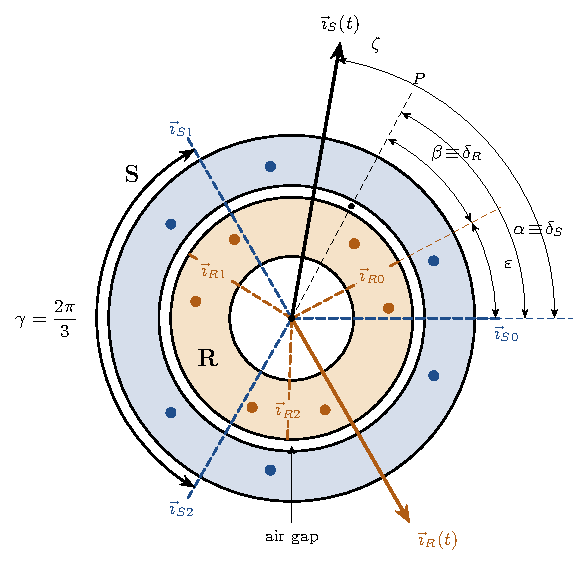
\includegraphics[width=0.62\linewidth]{figs/fig1-machine.pdf}
\caption{Cross-section of a symmetric three-phase AC machine, with the respective stator and rotor windings distributed and separated by the air gap. Redrawn after Leonhard~[1, Fig.~10.2a].}
\label{fig:machine}
\end{figure}

\section*{III. Development of the Vectorial AC Motor Model}

The progressive development of the vectorial model of the asynchronous AC motor is presented below, starting from the reference complex-domain model.

\subsection*{A. Geometric definitions and mathematical relations}

Geometric angle of displacement between coils:
\begin{equation}\tag{1}\label{eq:1}
\gamma = \tfrac{2}{3}\,\pi
\end{equation}

Angular coordinate of the stator (S) relative to the central axis of coil~0 of S:
\begin{equation}\tag{2}\label{eq:2}
\delta_0 \equiv \delta_S \equiv \alpha
\end{equation}

Angular coordinate of the rotor (R) relative to the central axis of coil~0 of R:
\begin{equation}\tag{3}\label{eq:3}
\delta_1 \equiv \delta_R \equiv \beta
\end{equation}

$\varepsilon(t)$: angle of rotation of R relative to the central axis of coil~0 of S. With this we establish the angle relation in the motor:
\begin{equation}\tag{4}\label{eq:4}
\delta_0 = \delta_1 + \varepsilon(t) \equiv \delta_S = \delta_R + \varepsilon(t) \equiv \alpha = \beta + \varepsilon(t)
\end{equation}
\begin{equation}\tag{5}\label{eq:5}
\delta_k = \delta_{k+1} + (-1)^k\,\varepsilon(t)
\end{equation}

Relation between the product of complex numbers and the scalar (dot) product of vectors [2]:
\begin{equation}\tag{6}\label{eq:6}
AB^{*} + A^{*}B = (a+jb)(c-jd) + (a-jb)(c+jd) = 2(ac+bd)
\end{equation}
\begin{equation}\tag{7}\label{eq:7}
A,B\in\mathbb{C}\;\Rightarrow\; AB^{*}+A^{*}B = 2\,\vec A\bullet\vec B\;\Leftarrow\;\vec A,\vec B\in\mathbb{R}^{2}
\end{equation}

Relation between the product of complex numbers and the cross vector product [2]:
\begin{equation}\tag{8}\label{eq:8}
AB^{*} - A^{*}B = (a+jb)(c-jd) - (a-jb)(c+jd) = j\,2\,(bc-ad)
\end{equation}
\begin{equation}\tag{9}\label{eq:9}
A,B\in\mathbb{C}\;\Rightarrow\; AB^{*}-A^{*}B = j\,2\,\vec A\times\vec B\;\Leftarrow\;\vec A,\vec B\in\mathbb{R}^{2}
\end{equation}

Relation between trigonometric functions, complex numbers, and vectors, using \eqref{eq:7}:
\begin{equation}\tag{10}\label{eq:10}
\cos(\delta) = \frac{e^{j\delta}+e^{-j\delta}}{2}
\end{equation}
\begin{equation}\tag{11}\label{eq:11}
\cos(\delta-\gamma) = \frac{e^{j(\delta-\gamma)}+e^{-j(\delta-\gamma)}}{2} = \frac{e^{j\delta}e^{-j\gamma}+e^{-j\delta}e^{j\gamma}}{2}
\end{equation}
\begin{equation}\tag{12}\label{eq:12}
\cos(\delta-\gamma) = e^{j\delta}\bullet e^{j\gamma}
\end{equation}

\subsection*{B. Current balance equation}

Balance equation for the currents of the electrical system:
\begin{equation}\tag{13}\label{eq:13}
\sum_n i_{kn}(t) = 0
\end{equation}
\begin{equation}\tag{14}\label{eq:14}
k:\{0,1\}\equiv\{S,R\}\ ;\qquad k+1=0\ \text{for}\ k=1
\end{equation}

$k$ is defined over the ring $\{0,1\}$, so $k+1=0$ for $k=1$.
\begin{equation}\tag{15}\label{eq:15}
n:\{0,1,2\}\equiv\{R,S,T\}\equiv\{a,b,c\}
\end{equation}

\subsection*{C. Definition of the stator and rotor current space vector}

Definition of the current space vector of S and R (Fig.~\ref{fig:spacevector}):
\begin{equation}\tag{16}\label{eq:16}
\vec\imath_k(t) = \sum_n i_{kn}(t)\,e^{jn\gamma}
\end{equation}

Alternative definition of the current space vector of S and R:
\begin{equation}\tag{17}\label{eq:17}
\vec\imath_k(t) = \sum_n i_{kn}(t)\,e^{jn\gamma} = i_k(t)\,e^{j\zeta_k(t)}
\end{equation}

$\zeta_k(t)$: angle of rotation of $\vec\imath_k(t)$ relative to the central axis of coil~0 of $k$.

\paragraph{Explicit deduction of $\zeta_k(t)$ from \eqref{eq:16}--\eqref{eq:17}.}

The angle $\zeta_k(t)$ is not an additional unknown of the model: it is deduced by equating the two definitions of the space vector, \eqref{eq:16} and \eqref{eq:17}, and separating real and imaginary parts. Expanding \eqref{eq:16} term by term:
\begin{equation}\tag{18}\label{eq:18}
\vec\imath_k(t) = i_{k0}(t)\,e^{j0} + i_{k1}(t)\,e^{j\gamma} + i_{k2}(t)\,e^{j2\gamma}
\end{equation}

with $\gamma=2\pi/3$, so the two complex roots involved are:
\begin{equation}\tag{19}\label{eq:19}
e^{j\gamma} = -\frac12 + j\frac{\sqrt3}{2}\ ,\qquad e^{j2\gamma} = -\frac12 - j\frac{\sqrt3}{2}
\end{equation}

Separating the real and imaginary parts of $\vec\imath_k(t)$:
\begin{equation}\tag{20}\label{eq:20}
\mathrm{Re}\{\vec\imath_k(t)\} = i_{k0}(t) - \tfrac12\, i_{k1}(t) - \tfrac12\, i_{k2}(t)
\end{equation}
\begin{equation}\tag{21}\label{eq:21}
\mathrm{Im}\{\vec\imath_k(t)\} = \frac{\sqrt3}{2}\,[\,i_{k1}(t) - i_{k2}(t)\,]
\end{equation}

The current balance condition \eqref{eq:13} implies that the sum of phases 1 and 2 is equal and opposite to phase~0:
\begin{equation}\tag{22}\label{eq:22}
i_{k1}(t) + i_{k2}(t) = -\,i_{k0}(t)
\end{equation}

with which the real part simplifies to:
\begin{equation}\tag{23}\label{eq:23}
\mathrm{Re}\{\vec\imath_k(t)\} = i_{k0}(t) - \tfrac12\bigl(-i_{k0}(t)\bigr) = \tfrac32\, i_{k0}(t)
\end{equation}

resulting in the form equivalent to the Clarke ($\alpha$-$\beta$) transform, written as a complex number:
\begin{equation}\tag{24}\label{eq:24}
\vec\imath_k(t) = \tfrac32\, i_{k0}(t) + j\,\frac{\sqrt3}{2}\,[\,i_{k1}(t) - i_{k2}(t)\,]
\end{equation}

Equating this expression with the polar form \eqref{eq:17} ---$i_k(t)e^{j\zeta_k(t)} = i_k(t)\cos\zeta_k(t)\allowbreak{} + j\,i_k(t)\sin\zeta_k(t)$--- component by component:
\begin{equation}\tag{25}\label{eq:25}
i_k(t)\cos\zeta_k(t) = \tfrac32\, i_{k0}(t)\ ,\qquad i_k(t)\sin\zeta_k(t) = \frac{\sqrt3}{2}\,[\,i_{k1}(t) - i_{k2}(t)\,]
\end{equation}

Dividing both expressions cancels $i_k(t)$, and $\zeta_k(t)$ is obtained explicitly as a function of the three phase currents (atan2 is used instead of plain arctan to preserve the correct quadrant, since $i_{k0}$ can be negative):
\begin{equation}\tag{26}\label{eq:26}
\zeta_k(t) = \operatorname{atan2}\Bigl(\frac{\sqrt3}{2}\,[\,i_{k1}(t) - i_{k2}(t)\,],\ \tfrac32\, i_{k0}(t)\Bigr)
\end{equation}

And along the way, dividing instead by the cosine or the sine and summing the squares, the magnitude is also determined:
\begin{equation}\tag{27}\label{eq:27}
i_k(t) = \frac32\sqrt{\,i_{k0}^{2}(t) + \tfrac13\,[\,i_{k1}(t) - i_{k2}(t)\,]^{2}}
\end{equation}

\begin{quote}\emph{Alternative physical verification.} From \eqref{eq:28h}, $\Theta_k(\delta_k,t)=N_k\,i_k(t)\cos[\zeta_k(t)-\delta_k]$ is a traveling cosine wave in the spatial variable $\delta_k$. Its maximum ---the crest of the mmf wave at instant $t$--- occurs exactly where the derivative with respect to $\delta_k$ vanishes:\end{quote}
\begin{equation}\tag{28}\label{eq:28}
\frac{\partial\Theta_k}{\partial\delta_k} = 0\ \Rightarrow\ \sin[\zeta_k(t)-\delta_k] = 0\ \Rightarrow\ \delta_k = \zeta_k(t)
\end{equation}

\begin{quote}\emph{That is: $\zeta_k(t)$ is, at each instant, the angular position where the mmf wave of winding $k$ reaches its maximum value along the air gap --- the same geometric interpretation shown by Fig.~\ref{fig:spacevector} as the angle of the resultant vector from the geometric sum of the three phase currents. Both paths, the algebraic one via the Clarke transform and the physical one via the maximum of the traveling wave, are mutually consistent and confirm that $\zeta_k(t)$ is fully determined by $i_{k0}(t)$, $i_{k1}(t)$, and $i_{k2}(t)$.}\end{quote}

\begin{figure}[htbp]
\centering
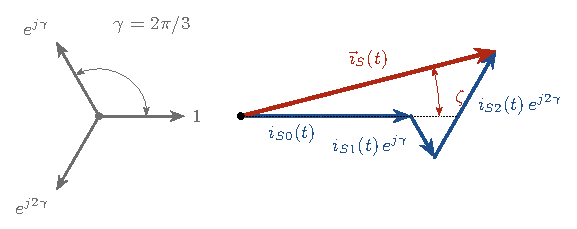
\includegraphics[width=0.7\linewidth]{figs/fig2-spacevector.pdf}
\caption{Current space vector as the geometric sum of the stator winding currents, for the instantaneous balanced values $(i_{S0},i_{S1},i_{S2})=(1.8,-0.5,-1.3)$. Redrawn after Leonhard~[1, Fig.~10.3a].}
\label{fig:spacevector}
\end{figure}

\subsection*{D. Calculation of the stator and rotor mmf}

Calculation of the magnetomotive force of the stator (S) and rotor (R). This forms a traveling wave, as shown in Fig.~\ref{fig:mmf}.
\begin{equation}\tag{28a}\label{eq:28a}
\Theta_k(\delta_k,t) = N_k\sum_n i_{kn}(t)\,\vartheta(\delta_k - n\gamma)
\end{equation}
\begin{equation}\tag{28b}\label{eq:28b}
-1 \le \vartheta(\delta_k - n\gamma) \le +1
\end{equation}

$\vartheta(\delta_k-n\gamma)$: spatial distribution function of the magnetomotive force of winding $n$, as a function of the stator or rotor measurement angle $\delta_k$. See Fig.~\ref{fig:distribution}.

\begin{figure}[htbp]
\centering
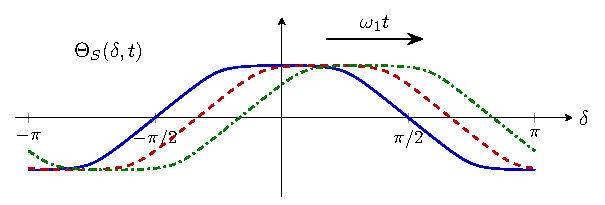
\includegraphics[width=0.8\linewidth]{figs/fig3-mmf.pdf}
\caption{Traveling magnetomotive-force wave of the stator, resulting from combining the contributions of its individual windings. Redrawn after Leonhard~[1, Fig.~10.2d].}
\label{fig:mmf}
\end{figure}

\begin{figure}[htbp]
\centering
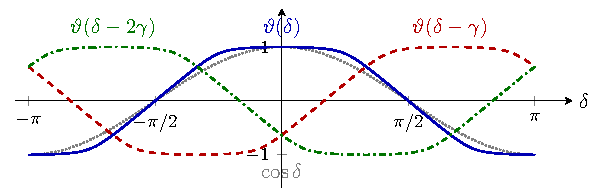
\includegraphics[width=0.8\linewidth]{figs/fig4-distribution.pdf}
\caption{Distribution functions of the magnetomotive force of the stator windings. Redrawn after Leonhard~[1, Fig.~10.2c].}
\label{fig:distribution}
\end{figure}

A harmonic-elimination approximation is made:
\begin{equation}\tag{28c}\label{eq:28c}
\vartheta(\delta_k - n\gamma) \cong \cos(\delta_k - n\gamma)
\end{equation}

Applying the previous relations and definitions to the mmf \eqref{eq:4} of S and R:
\begin{equation}\tag{28d}\label{eq:28d}
\Theta_k(\delta_k,t) = N_k\sum_n i_{kn}(t)\cos(\delta_k - n\gamma)
\end{equation}
\begin{equation}\tag{28e}\label{eq:28e}
\Theta_k(\delta_k,t) = N_k\sum_n i_{kn}(t)\,\bigl(e^{j\delta_k}\bullet e^{jn\gamma}\bigr)
\end{equation}
\begin{equation}\tag{28f}\label{eq:28f}
\Theta_k(\delta_k,t) = N_k\, e^{j\delta_k}\bullet\Bigl[\sum_n i_{kn}(t)\,e^{jn\gamma}\Bigr]
\end{equation}
\begin{equation}\tag{28g}\label{eq:28g}
\Theta_k(\delta_k,t) = N_k\,\vec\imath_k(t)\bullet e^{j\delta_k}
\end{equation}

Alternative definition of $\Theta_k(t)$:
\begin{equation}\tag{28h}\label{eq:28h}
\Theta_k(\delta_k,t) = N_k\, i_k(t)\cos[\zeta_k(t)-\delta_k]
\end{equation}

Given that by \eqref{eq:12}:
\begin{equation}\tag{28i}\label{eq:28i}
\cos(\zeta-\delta) = e^{j\zeta}\bullet e^{j\delta}
\end{equation}

We obtain:
\begin{equation}\tag{28j}\label{eq:28j}
\Theta_k(\delta_k,t) = N_k\, i_k(t)\,\bigl[e^{j\zeta_k(t)}\bullet e^{j\delta_k}\bigr]
\end{equation}

And the total mmf:
\begin{equation}\tag{28k}\label{eq:28k}
\Theta(t) = \sum_k \Theta_k(\delta_k,t)
\end{equation}

\subsection*{E. Calculation of the stator and rotor magnetic induction}

Magnetic induction or magnetic flux density in S or R due to the joint mmfs, using the angle relation between stator and rotor \eqref{eq:5}:
\begin{equation}\tag{29}\label{eq:29}
B_k\bigl(\delta_k,\varepsilon(t),t\bigr) = \frac{1}{2h}\,\mu_0\Bigl\{(1+\sigma_k)\,\Theta_k(\delta_k,t) + \Theta_{k+1}\bigl[\delta_k - (-1)^k\varepsilon(t),\,t\bigr]\Bigr\}
\end{equation}

Equivalent form as a function of each member's own angles:
\begin{equation}\tag{29b}\label{eq:29b}
B_k\bigl(\delta_k,\delta_{k+1},t\bigr) = \frac{1}{2h}\,\mu_0\Bigl[(1+\sigma_k)\,\Theta_k(\delta_k,t) + \Theta_{k+1}(\delta_{k+1},t)\Bigr]
\end{equation}

where $h$ is the air-gap thickness and $\sigma_k$ are the magnetic losses of S or R:
\begin{equation}\tag{29c}\label{eq:29c}
0 \le \sigma_k < 1
\end{equation}

\subsection*{F. Self and mutual inductances --- complete derivation}

The original paper presents this result as a direct consequence of ``integrating the inductive couplings or flux linkages,'' without developing it. That step is completed here. The method is the usual ``winding function'' one: the flux linked by phase $n$ of member $k$ is obtained by integrating the induction $B_k$ over the air gap, weighted by the distribution function (or ``pickup function'') of that same coil. For a two-pole distributed winding, this pickup function has amplitude $N_k/2$ ---half the amplitude $N_k$ used in the mmf \eqref{eq:28a}, the standard distinction between the ``turns function'' (for the mmf) and the ``winding function'' (for the flux linkage)--- so that:
\begin{equation}\tag{29d}\label{eq:29d}
\psi_{kn}(t) = \frac{N_k}{2}\,r\,\ell\int_0^{2\pi} B_k\bigl(\delta_k,\varepsilon(t),t\bigr)\cos(\delta_k - n\gamma)\,d\delta_k
\end{equation}

Using the product-to-sum trigonometric identity:
\begin{equation}\tag{29e}\label{eq:29e}
\int_0^{2\pi}\cos(\delta_k - m\gamma)\cos(\delta_k - n\gamma)\,d\delta_k = \pi\cos[(m-n)\gamma]
\end{equation}

\emph{Self term.} Substituting \eqref{eq:29b} for $B_k$ and applying the previous identity to the $(1+\sigma_k)\Theta_k$ part, together with the balanced-current condition \eqref{eq:13}, gives the identity:
\begin{equation}\tag{29f}\label{eq:29f}
\sum_m i_{km}(t)\cos[(m-n)\gamma] = \tfrac32\, i_{kn}(t)
\end{equation}

with which the self term of the flux linkage becomes:
\begin{equation}\tag{30}\label{eq:30}
\tfrac13 L_k = \frac{(1+\sigma_k)\,N_k^{2}\,\ell\, r\,\pi\,\mu_0}{8h}
\end{equation}

which reproduces exactly the result of the original paper.

\emph{Mutual term.} Similarly, with $\varphi\equiv(-1)^k\varepsilon(t)$, the same product-to-sum integral over the contribution of member $k+1$ gives:
\begin{equation}\tag{30a}\label{eq:30a}
\sum_p i_{k+1,p}(t)\cos[\varphi-(n-p)\gamma] = \bigl[\vec\imath_{k+1}(t)\,e^{j\varphi}\bigr]\bullet e^{jn\gamma},\qquad \varphi\equiv(-1)^k\varepsilon(t)
\end{equation}

which ---after reconstituting the current space vector of member $k+1$ and comparing with the expected form of equation \eqref{eq:32} below--- determines the mutual inductance:
\begin{equation}\tag{31}\label{eq:31}
\tfrac13 M = \frac{N_k\,N_{k+1}\,\ell\, r\,\pi\,\mu_0}{8h}
\end{equation}

Both results \eqref{eq:30} and \eqref{eq:31} share the same denominator $8h$, and their ratio $L_k/M=(1+\sigma_k)N_k/N_{k+1}$ is identical to the one obtained by Leonhard's classical scalar path, which confirms the consistency of the vectorial model with the original complex model.

\subsection*{G. Calculation of the stator and rotor inductive couplings}

Using \eqref{eq:30} and \eqref{eq:31}, the inductive couplings of stator and rotor take the following vectorial form:
\begin{equation}\tag{32}\label{eq:32}
\psi_{kn}(t) = \tfrac23\Bigl\{L_k\,\vec\imath_k(t)\bullet e^{jn\gamma} + M\,\vec\imath_{k+1}(t)\bullet e^{j[n\gamma-(-1)^k\varepsilon(t)]}\Bigr\}
\end{equation}

\subsection*{H. Definition of the inductive-coupling space vector --- complete derivation}

Definition of the inductive-coupling space vector of S and R:
\begin{equation}\tag{33}\label{eq:33}
\vec\psi_k(t) = \sum_n \psi_{kn}(t)\,e^{jn\gamma}
\end{equation}

Substituting \eqref{eq:32} into \eqref{eq:33}:
\begin{equation}\tag{34}\label{eq:34}
\vec\psi_k(t) = \sum_n \tfrac23\Bigl\{L_k\,\vec\imath_k(t)\bullet e^{jn\gamma} + M\,\vec\imath_{k+1}(t)\bullet e^{j[n\gamma-(-1)^k\varepsilon(t)]}\Bigr\}\,e^{jn\gamma}
\end{equation}

The original paper summarizes this step as ``after some algebraic elaboration.'' That elaboration is completed here by means of a three-phase collapse lemma, a direct consequence of the system's $120^\circ$ symmetry (the same kind of cancellation that underlies the current balance \eqref{eq:13}--\eqref{eq:15}):
\begin{equation}\tag{34a}\label{eq:34a}
\sum_{n=0}^{2}\tfrac23\,\bigl(A\bullet e^{jn\gamma}\bigr)\,e^{jn\gamma} = A\qquad\Bigl(\gamma=\frac{2\pi}{3}\Bigr)
\end{equation}

\emph{Proof of the lemma.} For any $A\in\mathbb{C}$ constant in $n$, the dot product can be written as a real part:
\begin{equation}\tag{34b}\label{eq:34b}
A\bullet e^{jn\gamma} = \mathrm{Re}\bigl(A\,e^{-jn\gamma}\bigr) = \frac{A\,e^{-jn\gamma} + A^{*}e^{jn\gamma}}{2}
\end{equation}

multiplying by $(2/3)e^{jn\gamma}$:
\begin{equation}\tag{34c}\label{eq:34c}
\tfrac23\bigl(A\bullet e^{jn\gamma}\bigr)\,e^{jn\gamma} = \tfrac13\bigl(A + A^{*}e^{j2n\gamma}\bigr)
\end{equation}

and summing over $n=0,1,2$:
\begin{equation}\tag{34d}\label{eq:34d}
\sum_{n=0}^{2}\tfrac13\bigl(A + A^{*}e^{j2n\gamma}\bigr) = A + \frac{A^{*}}{3}\sum_{n=0}^{2} e^{j2n\gamma}
\end{equation}

With $\gamma=2\pi/3$, the exponent $2n\gamma$ runs over the three cube roots of unity, whose sum is identically zero:
\begin{equation}\tag{34e}\label{eq:34e}
\sum_{n=0}^{2} e^{jn\frac{4\pi}{3}} = 1 + e^{j\frac{4\pi}{3}} + e^{j\frac{8\pi}{3}} = 0
\end{equation}

so the second term vanishes and the whole sum collapses exactly to $A$, proving the lemma above.

Application to the self term of \eqref{eq:34}, with $A=L_k\vec\imath_k(t)$ (constant in $n$):
\begin{equation}\tag{34f}\label{eq:34f}
\sum_n \tfrac23\bigl[L_k\,\vec\imath_k(t)\bullet e^{jn\gamma}\bigr]e^{jn\gamma} = L_k\,\vec\imath_k(t)
\end{equation}

Application to the mutual term. First bringing the exponent to the pure $e^{jn\gamma}$ form via a phase shift $\varphi$:
\begin{equation}\tag{34g}\label{eq:34g}
B\bullet e^{j(n\gamma-\varphi)} = \bigl(B\,e^{j\varphi}\bigr)\bullet e^{jn\gamma}
\end{equation}

with $B=\vec\imath_{k+1}(t)$ and $\varphi=(-1)^k\varepsilon(t)$, the term is also constant in $n$ and the lemma applies directly:
\begin{equation}\tag{34h}\label{eq:34h}
\sum_n \tfrac23\Bigl[M\,\vec\imath_{k+1}(t)\,e^{j(-1)^k\varepsilon(t)}\bullet e^{jn\gamma}\Bigr]e^{jn\gamma} = M\,\vec\imath_{k+1}(t)\,e^{j(-1)^k\varepsilon(t)}
\end{equation}

Summing both results gives exactly the result stated in the original paper:
\begin{equation}\tag{35}\label{eq:35}
\vec\psi_k(t) = L_k\,\vec\imath_k(t) + M\,\vec\imath_{k+1}(t)\,e^{j(-1)^k\varepsilon(t)}
\end{equation}

The trigonometric sum over the three phases cancels completely thanks to the $120^\circ$ geometric phase shift between windings: the flux-linkage space vector is expressed as the superposition of the self flux with the mutual flux coupled from the other winding, rotated by the corresponding mechanical angle.

Angular speed of the mmf of $k\in\{S,R\}$:
\begin{equation}\tag{36}\label{eq:36}
\omega_k(t) = \dot\zeta_k(t)
\end{equation}

Angular speed of the motor of $k\in\{S,R\}$:
\begin{equation}\tag{37}\label{eq:37}
\omega_M(t) = \dot\varepsilon(t)
\end{equation}

\begin{quote}\emph{Note: \eqref{eq:37} is not obtained algebraically from \eqref{eq:36}, but by analogical extension of the same definition ---angular speed as the time derivative of a rotation angle--- to the mechanical angle $\varepsilon(t)$ already defined in \eqref{eq:4}--\eqref{eq:5}, instead of the electrical angle $\zeta_k(t)$. Both angles describe a rotation relative to a fixed reference axis, but one is electrical and the other mechanical; they are not in general equal or proportional to each other without additional information (hence the slip in the induction machine).}\end{quote}

\subsection*{I. Calculation of the stator and rotor voltages}

Analogously, what was done can be applied to the voltage equation of S and R:
\begin{equation}\tag{38}\label{eq:38}
u_{kn}(t) = R_k\, i_{kn}(t) + \dot\psi_{kn}(t)
\end{equation}

\subsection*{J. Definition of the stator and rotor voltage space vector}

Definition of the voltage space vector of S and R:
\begin{equation}\tag{39}\label{eq:39}
\vec u_k(t) = \sum_n u_{kn}(t)\,e^{jn\gamma}
\end{equation}

\subsection*{K. Torque equation --- complete derivation and sign correction}

Torque equation according to W.~Leonhard:
\begin{equation}\tag{40}\label{eq:40}
T_M(t) = \frac{M}{3\pi}\int_0^{2\pi}\frac{i_S\,i_R^{*}\,e^{-j\varepsilon(t)} - i_S^{*}\,i_R\,e^{j\varepsilon(t)}}{2j}\,d\beta
\end{equation}

The integrand does not depend on $\beta$, so the integral is resolved as the integrand multiplied by $2\pi$:
\begin{equation}\tag{41}\label{eq:41}
T_M(t) = \tfrac23\,M\cdot\frac{i_S\,i_R^{*}\,e^{-j\varepsilon} - i_S^{*}\,i_R\,e^{j\varepsilon}}{2j}
\end{equation}

We define $W\equiv i_S(t)\cdot i_R^{*}(t)\cdot e^{-j\varepsilon(t)}$ (where $i_S\equiv i_0$ and $i_R\equiv i_1$ in the general notation of this section), with which $W^{*}=i_S^{*}(t)\cdot i_R(t)\cdot e^{j\varepsilon(t)}$, and since $(W-W^{*})/(2j)=\mathrm{Im}\{W\}$:
\begin{equation}\tag{41a}\label{eq:41a}
W \equiv i_S(t)\,i_R^{*}(t)\,e^{-j\varepsilon(t)}\ ,\qquad W^{*} = i_S^{*}(t)\,i_R(t)\,e^{j\varepsilon(t)}
\end{equation}
\begin{equation}\tag{41b}\label{eq:41b}
\frac{W - W^{*}}{2j} = \mathrm{Im}\{W\}
\end{equation}

the intermediate form given in the original paper is obtained:
\begin{equation}\tag{42}\label{eq:42}
T_M(t) = \tfrac23\,M\,\mathrm{Im}\bigl\{i_S(t)\,\bigl[i_R(t)\,e^{j\varepsilon(t)}\bigr]^{*}\bigr\}
\end{equation}

Identity \eqref{eq:9} is now applied, defining $A=i_S(t)$ and $B=i_R(t)\cdot e^{j\varepsilon(t)}$. First we verify that $A\cdot B^{*}$ coincides exactly with $W$:
\begin{equation}\tag{42a}\label{eq:42a}
AB^{*} = i_S(t)\,\bigl[i_R(t)\,e^{j\varepsilon(t)}\bigr]^{*} = W\qquad\checkmark
\end{equation}

and since $\mathrm{Im}(AB^{*})$ is precisely the left-hand side of identity \eqref{eq:9}:
\begin{equation}\tag{42b}\label{eq:42b}
\mathrm{Im}(AB^{*}) = \frac{AB^{*} - A^{*}B}{2j} = \vec A\times\vec B
\end{equation}

we obtain:
\begin{equation}\tag{43}\label{eq:43}
T_M(t) = \tfrac23\,M\Bigl[\vec\imath_S(t)\times\vec\imath_R(t)\,e^{+j\varepsilon(t)}\Bigr]
\end{equation}

\begin{quote}\emph{Sign correction. The original text of this publication presents the final equation as:}\end{quote}
\begin{equation}\tag{43a}\label{eq:43a}
\vec T_M(t)\ \textbf{(original text)}:\quad \tfrac23\,M\Bigl[\vec\imath_S(t)\times\vec\imath_R(t)\,e^{-j\varepsilon(t)}\Bigr]
\end{equation}

\begin{quote}\emph{that is, with exponent $-\varepsilon(t)$. Mechanically applying the only tool the paper itself offers for this step ---identity \eqref{eq:9}--- the sign that results from the complete derivation is $+\varepsilon(t)$, not $-\varepsilon(t)$. Since the derivation \eqref{eq:40}--\eqref{eq:43} is a closed, step-by-step verifiable algebraic chain starting from Leonhard's own equation, \eqref{eq:43} is adopted here as the corrected form, and the discrepancy is attributed to a transcription error of the exponent's sign in the original document. This correction was additionally verified mechanically using the ACL2 theorem prover ---independently of the algebraic development presented here--- obtaining exactly the same sign $+\varepsilon(t)$~[3].}\end{quote}

\subsection*{L. Final model of the asynchronous AC machine}

Introducing equivalence \eqref{eq:9}, the final model of the asynchronous AC machine is:
\begin{equation}\tag{44}\label{eq:44}
\vec u_k(t) = R_k\,\vec\imath_k(t) + \dot{\vec\psi}_k(t)
\end{equation}
\begin{equation}\tag{45}\label{eq:45}
J\,\dot{\vec\omega}_M(t) = \vec T_M(t) - \vec T_L(t)
\end{equation}
\begin{equation}\tag{46}\label{eq:46}
\vec T_M(t) = \tfrac23\,M\Bigl[\vec\imath_S(t)\times\vec\imath_R(t)\,e^{+j\varepsilon(t)}\Bigr]
\end{equation}

\begin{quote}\emph{Equation \eqref{eq:46} reproduces exactly \eqref{eq:43} ---both already with the corrected sign, unlike the equation with the original text shown above only for comparison purposes--- and closes the model: $J$ is the rotor's moment of inertia, $\vec T_L(t)$ the external load torque.}\end{quote}

\section*{IV. Conclusion}

The development of the asynchronous AC machine has been presented starting from the complex-domain model, from which a vectorial model was obtained that reveals the nature of the motor torque as a cross vector product of the rotating stator and rotor current vectors. Relative to the original publication, this version completes three derivations that were left implicit there ---the self and mutual inductances, the three-phase collapse of the flux linkage, and the complete chain leading to the torque equation--- and corrects, with explicit algebraic justification and independent mechanical verification via ACL2~[3], the sign of the exponent in the final torque equation. The use of this representation is proposed for educational purposes, where the explanation of current interaction is made graphical through vector operations, and it can also be evaluated numerically, being equivalent to the original complex model from which it was derived.

\subsection*{Future Work}

The symbolic verification originally planned using a computer-algebra system such as Maxima was replaced by a more rigorous formal verification: the algebraic core of the model ---the identities \eqref{eq:6}--\eqref{eq:9}, the three-phase collapse lemma of Section~III.H, and the complete chain of the torque sign correction of Section~III.K--- was mechanically proved in ACL2, including a concrete instantiation with real $\gamma=2\pi/3$ via ACL2(r)~[3]. It remains to formalize in the same way the integration of the self and mutual inductances (Section~III.F), for which the real integral-calculus library of ACL2(r) (\texttt{nonstd/integrals}) has already been identified as the formalization path, and the exact antiderivative needed was obtained by hand; the mechanization of the differentiation step remains. Numerical verification of the complete model ---including the corrected torque sign--- via Scilab simulation also remains pending.

\section*{V. Cross-reference to the ACL2 books}

The ACL2 books are in the ACL2 community books, directory \texttt{books/\allowbreak workshops/\allowbreak 2026/\allowbreak cayuela-\allowbreak ac-\allowbreak machine/}~[3]. The first table gives, for each theorem, the equation(s) of this appendix that it states or proves. Theorems that only support a proof (arithmetic lemmas) are not listed.

\begin{longtable}{@{}>{\raggedright\arraybackslash}p{0.50\linewidth}>{\raggedright\arraybackslash}p{0.46\linewidth}@{}}
\toprule
Theorem & Equation(s)\\
\midrule
\endhead
\multicolumn{2}{@{}l}{\textit{00-\allowbreak complex-\allowbreak vectors.lisp}}\\
\quad \texttt{eq6-\allowbreak dot-\allowbreak product-\allowbreak real-\allowbreak part}, \texttt{eq6-\allowbreak dot-\allowbreak product-\allowbreak imag-\allowbreak part} & (6), (7)\\
\quad \texttt{eq8-\allowbreak 9-\allowbreak cross-\allowbreak product-\allowbreak real-\allowbreak part}, \texttt{eq8-\allowbreak 9-\allowbreak cross-\allowbreak product-\allowbreak imag-\allowbreak part} & (8), (9)\\
\quad \texttt{eq9-\allowbreak im-\allowbreak ab-\allowbreak star-\allowbreak is-\allowbreak crossp} & (9), (42b)\\
\multicolumn{2}{@{}l}{\textit{01-\allowbreak euler-\allowbreak identities.lisp}}\\
\quad \texttt{pythagorean-\allowbreak cos-\allowbreak sin}, \texttt{cosine-\allowbreak even}, \texttt{sine-\allowbreak odd}, \texttt{cosine-\allowbreak difference}, \texttt{sine-\allowbreak difference}, \texttt{acl2-\allowbreak numberp-\allowbreak cosine}, \texttt{acl2-\allowbreak numberp-\allowbreak sine} & assumed properties of $\cos$ and $\sin$ (\texttt{encapsulate}), used in (10)--(12) and (34g)\\
\quad \texttt{eq10-\allowbreak euler-\allowbreak cosine} & (10)\\
\quad \texttt{eq12-\allowbreak cosine-\allowbreak difference-\allowbreak is-\allowbreak dotp} & (12), through (11)\\
\multicolumn{2}{@{}l}{\textit{02-\allowbreak roots-\allowbreak of-\allowbreak unity.lisp}}\\
\quad \texttt{eq-\allowbreak roots-\allowbreak of-\allowbreak unity-\allowbreak sum-\allowbreak zero} & (19): $1+e^{j\gamma}+e^{j2\gamma}=0$\\
\quad \texttt{eq-\allowbreak roots-\allowbreak of-\allowbreak unity-\allowbreak double-\allowbreak angle-\allowbreak sum-\allowbreak zero} & (34e)\\
\multicolumn{2}{@{}l}{\textit{03-\allowbreak zeta-\allowbreak deduction.lisp}}\\
\quad \texttt{eq16-\allowbreak 28-\allowbreak re-\allowbreak ik-\allowbreak balanced} & (23)\\
\quad \texttt{eq16-\allowbreak 28-\allowbreak imz-\allowbreak ik} & (21)\\
\quad \texttt{eq-\allowbreak ik-\allowbreak magnitude-\allowbreak squared} & (27)\\
\multicolumn{2}{@{}l}{\textit{04-\allowbreak collapse-\allowbreak lemma.lisp}}\\
\quad \texttt{eq33-\allowbreak 35-\allowbreak three-\allowbreak phase-\allowbreak collapse-\allowbreak lemma} & (34a); its proof is (34b)--(34e), and its applications (34f), (34h)\\
\quad \texttt{eq-\allowbreak mutual-\allowbreak phase-\allowbreak shift} & (34g)\\
\multicolumn{2}{@{}l}{\textit{05-\allowbreak torque-\allowbreak sign-\allowbreak correction.lisp}}\\
\quad \texttt{eq-\allowbreak W-\allowbreak conjugate} & (41a): $W^{*}$\\
\quad \texttt{eq-\allowbreak w-\allowbreak minus-\allowbreak wconj-\allowbreak is-\allowbreak 2j-\allowbreak im} & (41b)\\
\quad \texttt{eq-\allowbreak ab-\allowbreak star-\allowbreak is-\allowbreak w} & (42a)\\
\quad \texttt{eq-\allowbreak im-\allowbreak w-\allowbreak is-\allowbreak crossp} & (42b), (43)\\
\quad \texttt{torque-\allowbreak exponent-\allowbreak sign-\allowbreak is-\allowbreak plus} & (43), against (43a)\\
\quad \texttt{sign-\allowbreak matters-\allowbreak nonvacuous} & (43) and (43a) differ: the sign matters\\
\multicolumn{2}{@{}l}{\textit{06-\allowbreak generic-\allowbreak omega-\allowbreak collapse.lisp}}\\
\quad \texttt{trinary-\allowbreak collapse-\allowbreak lemma} (and its supporting lemmas) & (34a), for any $\omega$ with $\omega^{2}+\omega+1=0$\\
\multicolumn{2}{@{}l}{\textit{06-\allowbreak generic-\allowbreak omega-\allowbreak collapse-\allowbreak acl2r.lisp}}\\
\quad \texttt{cos-\allowbreak gamma-\allowbreak val}, \texttt{sin-\allowbreak gamma-\allowbreak val}, \texttt{omega-\allowbreak real-\allowbreak closed-\allowbreak form}, \texttt{omega-\allowbreak real-\allowbreak satisfies-\allowbreak cubic} & (19): $\omega=e^{j2\pi/3}$\\
\quad \texttt{trinary-\allowbreak collapse-\allowbreak CONCRETE} & (34a), with $\omega=e^{j2\pi/3}$\\
\multicolumn{2}{@{}l}{\textit{07-\allowbreak inductance-\allowbreak note.lisp}}\\
\quad (no theorems) & (29)--(31): the integral (29e) is not mechanized\\
\multicolumn{2}{@{}l}{\textit{08-\allowbreak inductance-\allowbreak integral.lisp}}\\
\quad \texttt{cos-\allowbreak product-\allowbreak to-\allowbreak sum} & (29e): product-to-sum identity\\
\quad \texttt{inductance-\allowbreak integrand-\allowbreak as-\allowbreak sum} & (29e): integrand as a sum\\
\quad \texttt{sin-\allowbreak 2x-\allowbreak minus-\allowbreak c-\allowbreak deriv} & derivative of the antiderivative of (29e)\\
\multicolumn{2}{@{}l}{\textit{09-\allowbreak nonvacuity-\allowbreak acl2r.lisp}}\\
\quad \texttt{sqrt-\allowbreak 3-\allowbreak squared-\allowbreak nv}, \texttt{realp-\allowbreak sqrt-\allowbreak 3}, \texttt{s3-\allowbreak hypothesis-\allowbreak satisfiable} & (19): $\sqrt3$ is real with square 3\\
\quad \texttt{eq33-\allowbreak 35-\allowbreak collapse-\allowbreak concrete} & (34a)\\
\quad \texttt{eq-\allowbreak ik-\allowbreak magnitude-\allowbreak squared-\allowbreak concrete} & (27)\\
\quad \texttt{sign-\allowbreak matters-\allowbreak concrete} & (43), (43a)\\
\quad \texttt{acl2-\allowbreak trig-\allowbreak pythagorean}, \texttt{acl2-\allowbreak trig-\allowbreak cosine-\allowbreak even}, \texttt{acl2-\allowbreak trig-\allowbreak sine-\allowbreak odd}, \texttt{acl2-\allowbreak trig-\allowbreak cosine-\allowbreak difference}, \texttt{acl2-\allowbreak trig-\allowbreak sine-\allowbreak difference}, \texttt{acl2-\allowbreak trig-\allowbreak numberp-\allowbreak cosine}, \texttt{acl2-\allowbreak trig-\allowbreak numberp-\allowbreak sine} & the constraints of the \texttt{encapsulate}, proved for \texttt{acl2-cosine} and \texttt{acl2-sine}\\
\quad \texttt{eq10-\allowbreak euler-\allowbreak cosine-\allowbreak r}, \texttt{eq12-\allowbreak cosine-\allowbreak difference-\allowbreak is-\allowbreak dotp-\allowbreak r} & (10), (12)\\
\quad \texttt{eq-\allowbreak mutual-\allowbreak phase-\allowbreak shift-\allowbreak r} & (34g)\\
\quad \texttt{eq-\allowbreak W-\allowbreak conjugate-\allowbreak r} & (41a)\\
\quad \texttt{eq-\allowbreak im-\allowbreak w-\allowbreak is-\allowbreak crossp-\allowbreak r}, \texttt{torque-\allowbreak exponent-\allowbreak sign-\allowbreak is-\allowbreak plus-\allowbreak r} & (42b), (43)\\
\bottomrule
\end{longtable}

Some comments inside the books refer to ``images''. The source document of this appendix was written with every equation and figure as an image, numbered in order of appearance: figure~1 is image~1, so an equation has image number equal to its original position plus the figures before it. The second table translates those comments.

\begin{center}\small
\begin{tabular}{@{}p{0.47\linewidth}lp{0.34\linewidth}@{}}
\toprule
Comment in the book & Image & Equation(s)\\
\midrule
\texttt{02-roots-of-unity}: ``Image 20'' & 20 & (19), the two complex roots\\
\texttt{04-collapse-lemma}: ``images 56-60'' & 56--60 & (34a)--(34e), lemma and proof\\
\texttt{02-roots-of-unity}: ``images 58-60'' & 58--60 & (34c)--(34e)\\
\texttt{02-roots-of-unity}: ``Image 60'' & 60 & (34e), sum of the roots with the doubled angle\\
\texttt{04-collapse-lemma}: ``image 62'' & 62 & (34g), phase shift\\
\texttt{05-torque-sign-correction}: ``image 74'' & 74 & (42a), $AB^{*}=W$ with the check mark\\
\bottomrule
\end{tabular}
\end{center}


\section*{References}
\begin{description}\setlength{\itemsep}{0.1em}
\item[{[1]}] W.~Leonhard, \emph{Control of Electrical Drives}, 2nd and 3rd ed.\ Springer 1996--2001, Chapter~10, Symmetrical Three-Phase AC Machines.
\item[{[2]}] T.~Needham, \emph{Visual Complex Analysis}, 1st ed.\ Oxford: Clarendon Press, 2000, Ch.~1, Part~III, Section~6, Vectorial Operations.
\item[{[3]}] P.~O.~Cayuela, ``Mechanized Verification of Complex-to-Vector Derivations in a Three-Phase AC Machine Model,'' 20th International Workshop on the ACL2 Theorem Prover and Its Applications (ACL2-2026), EPTCS, to appear. The books are in the ACL2 community books, \texttt{[books]/workshops/2026/cayuela-ac-machine/}; development version: \url{https://github.com/pcayuela/ACL2-ACmotormodel-check}
\end{description}

\end{document}
